\setlength{\unitlength}{1pt}
\begin{picture}(0,0)
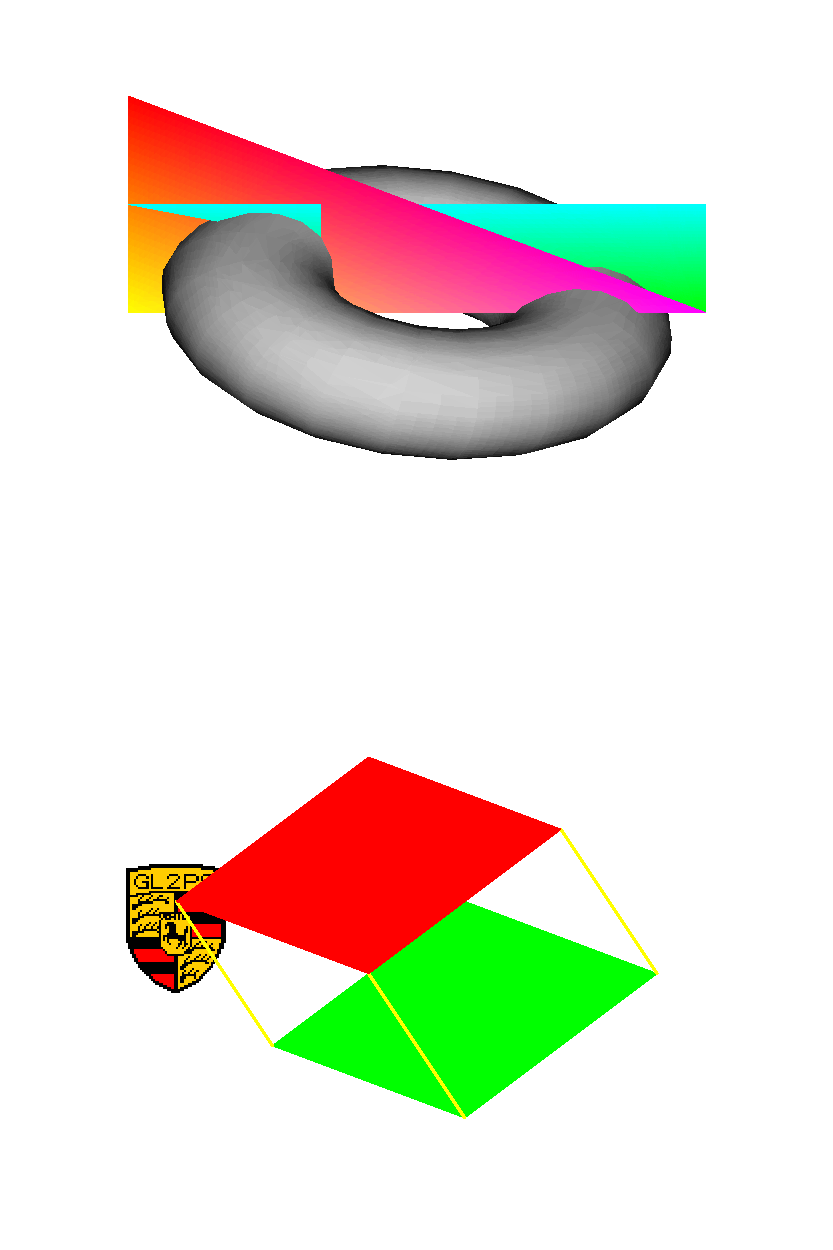
\includegraphics{outLatex}
\end{picture}%
\begin{picture}(400,600)(0,0)
\put(26.9229,389.769){\makebox(0,0)[lb]{Press:}}
\put(26.9229,376.269){\makebox(0,0)[lb]{  s: to save the images}}
\put(26.9229,362.769){\makebox(0,0)[lb]{  t: to alternate between teapot and torus}}
\put(26.9229,349.269){\makebox(0,0)[lb]{  v: to alternate between single and multiple viewport modes}}
\put(26.9229,335.769){\makebox(0,0)[lb]{  q: to quit}}
\put(26.9229,322.269){\makebox(0,0)[lb]{Click and move the mouse to rotate the objects}}
\end{picture}
